% smc.tex

\chapter{Sequential Monte Carlo for Free Energy Estimation}
\label{chap:smc}

Path optimization in free energy calculations comes in several forms. 
In chapter \ref{chap:dijkstra}, we explored the possibility of optimizing the intermediates that make up the path, in order to minimize the variance and decrease the required number of samples needed to reach a desired precision.
In this chapter, we will approach optimization from a complementary angle. 
Given a fixed alchemical path, can we reduce the computational cost per sample, and can we construct an efficient estimator with the minimum variance properties of BAR?

There is considerable overlap between chemical physics studies on free energy calculations and research in statistics for estimating ratios of normalizing constants. 
Indeed, as we pointed out with the relationship between BAR and bridge sampling, methods from the statistics literature have previously been adapted for use in biophysical problems.

Nonequilibrium methods, such as Jarzynski's method\cite{jarzynski1997nonequilibrium1}, have gone largely underappreciated in the chemical physics literature despite their statistical equivalent, sequential Monte Carlo\cite{cappe2007overview, del2006sequential} (SMC), enjoying widespread use.
A key benefit of SMC methods that we would like to leverage in molecular simulation is the enormous reduction in computational cost for sampling.
For equilibrium sampling, assuming a system relaxation time of $\tau$ and $k$ alchemical states in the path, to obtain $n$ draws would require $\mathcal{O}(\tau k n)$ computation.
On the other hand, for nonequilibrium sampling, we only require $\mathcal{O}(\tau n)$ time to generate initial configurations from one equilibrium simulation, then through a series of cheap nonequilibrium moves, we generate weighted particle trajectories in time $\mathcal{O}((k-1)\tau^\prime n)$, for a total cost of $\mathcal{O}((\tau + (k-1)\tau^\prime)n)$, where $\tau >> \tau^\prime$. 

\section{Combining bridge sampling and SMC}

The primary downside of Jarzynski's method and its statistical analogue, annealed important sampling\cite{neal2001annealed} (AIS), is that while the sample collection step is rapid, the ratio estimation step is inefficient. 
This is because these are one-sided estimators, which only use draws from one target state, of which the most well known is Zwanzig's exponential averaging\cite{zwanzig1954high}:

\begin{equation}
    \Delta G_{0 \rightarrow 1} = -\beta^{-1} \log E_0[\exp(-\beta(U_1(x)-U_0(x))]
\end{equation}

To remedy this statistical inefficiency, we develop a modified version of BAR, that we call sequential BAR (seqBAR, or sBAR), which uses the BAR estimation step with rapidly generated SMC particles.
This fusion of SMC and bridge sampling methods is enabled by a resampling step\cite{murray2012gpu}, which transforms weighted SMC particles into a collection of draws approximating the equilibrium distribution for every intermediate state.
These resampled particles can then be used directly in BAR estimation as in equation \eqref{bridgesam}. 

\begin{figure}
    \centering
    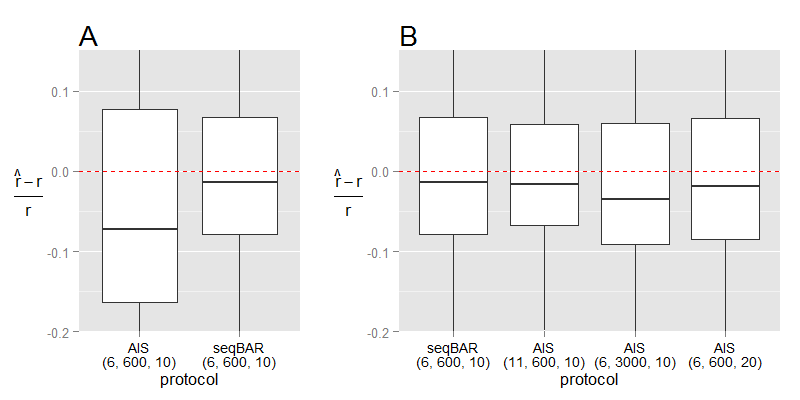
\includegraphics[scale=0.7]{seqBARvAIS-uni-bi-v02.png}
    \caption[Comparison of seqBAR and AIS performance for the normal to bimodal transformation]{Comparison of seqBAR and AIS performance for the normal to bimodal transformation. Performance is judged by the empirical accuracy and precision of the relative error of the ratio estimate for 500 independent realizations. Protocols are defined by an estimation method (AIS or seqBAR), followed by a trio of parameters, indicating respectively, the number of distributions in the path, the number of sample trajectories, and the number of Metropolis mixing steps per transition. Left panel: Comparison of AIS and seqBAR performance for equal computation time. Right panel: Required computation for AIS to match seqBAR performance.}
    \label{fig:sBARvAIS}
\end{figure}

Figure \ref{fig:sBARvAIS} demonstrates the gains in statistical efficiency when using seqBAR over AIS. 
For equal computation, seqBAR is, on average, closer to the true ratio value, and has more consistent ratio estimates, from replicate to replicate. 
To match the performance of seqBAR, AIS requires either a doubling of the number of distributions in the path, a five-fold increase in the number of samples, or a doubling in the cost of each nonequilibrium transition, here a Metropolis\cite{metropolis1953equation} mixing step.

\section{SMC in the augmented $(\lambda, T)$ space}
\label{sec:smcpath}

SMC methods are also sensitive to path choice. 
For the normal to normal example, five paths in the $(\lambda, T)$ space were compared using AIS. 
Ratio estimates, squared errors and estimated variances are shown in figure \ref{fig:AIS-pathcompare}.
We note that there appears to be a tradeoff with using the higher temperatures. 
As temperature increases up to a maximum value of 3 (a path height of 2), AIS performance improves. 
Once temperature increases beyond that point (path heights 3 and 4), the increased temperature introduces too much noise, and the variance of the ratio estimate increases, even beyond that of an AIS run using the standard, fixed temperature path.

\begin{figure}
    \centering
    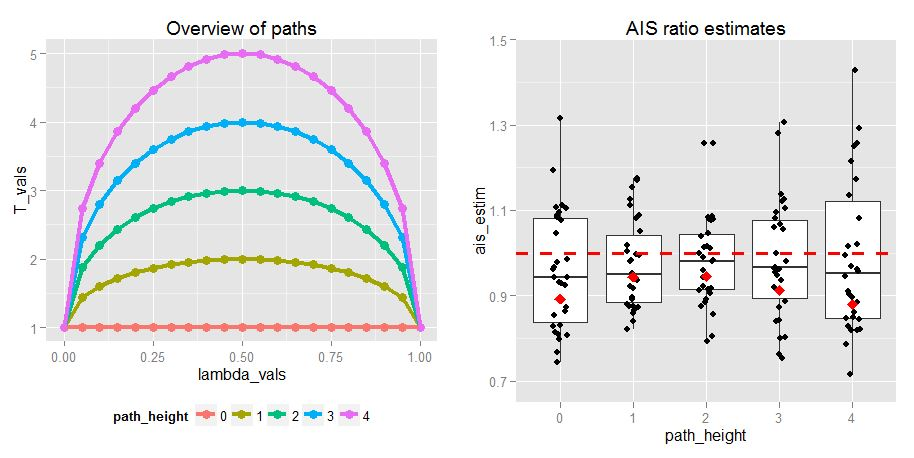
\includegraphics[scale=0.6]{ais-pathcompare.jpg}
    \caption[Comparison of AIS paths for offset harmonic wells]{Comparison of AIS paths for offset harmonic wells. Left: parameter space representation of paths. Right: ratio estimates indexed by path. The dotted red line denotes the true ratio. Red diamonds represent average values for each path height.}
    \label{fig:AIS-pathcompare}
\end{figure}

\section{pCrooks: a pairwise decomposable CFT}
\label{sec:pcrooks}

Regardless of path, there are conditions under which AIS and seqBAR can struggle, namely when the target distributions are sufficiently different such that nonequilibrium moves are unable to create particles approximating the final distribution. 
One such example is the transition from a normal distribution to a Cauchy distribution (t-distribution with one degree of freedom), due to their differing tail decay rates.
In the same way that BAR improves on exponential averaging by creating bridge functions and utilizing samples from both target distributions, the Crooks fluctuation theorem\cite{crooks2000path} (CFT) improves on Jarzynski's method. 
CFT is a a hybrid SMC-bridge sampling method, which operates on nonequilibrium work distributions generated in both sampling directions.
This bidirectional propagation results in increased robustness to varying target distributions for ratio estimation, as seen in figure \ref{fig:pcrooks}.
Note that both AIS and seqBAR are highly variable, and frequently under estimate the ratio, whereas CFT (crooks) is extremely accurate.

\begin{figure}
    \centering
    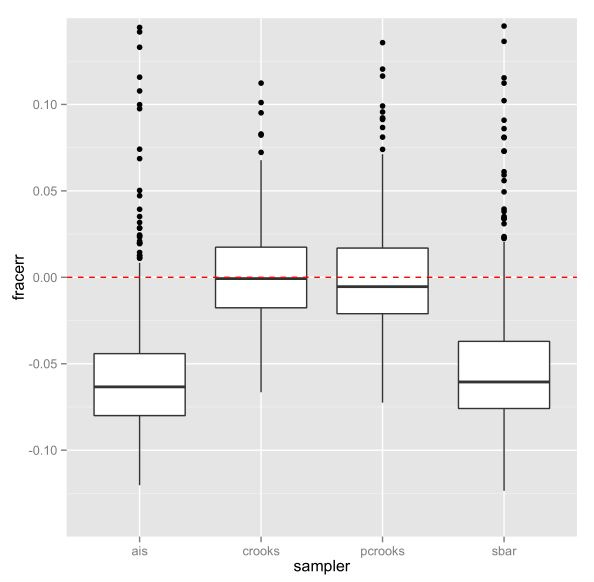
\includegraphics[scale=0.6]{pcrooks.jpg}
    \caption[Comparison of various SMC methods for the normal to Cauchy transformation]{Comparison of AIS, CFT, pCrooks and seqBAR ratio estimation performance for the normal to Cauchy distribution transformation.}
    \label{fig:pcrooks}
\end{figure}

In the context of path selection however, CFT has notable shortcomings. 
For path selection between enumerated (and frequently non-overlapping) paths, CFT is acceptable, but when trying to optimize paths in a full grid search, when there may be significant barriers to work around, and we have no guesses as to what form an acceptable path may take, the dependence on CFT on full path work distributions hinders our ability to locally optimize transitions and build reasonable paths.
To this end, we developed pairwise Crooks (pCrooks), a pairwise decomposable version of CFT. 
Instead of using full path work distributions to estimate the full telescoping ratio in one step, we calculate each pairwise ratio using BAR with weighted work distributions, where the weights are derived from the accumulated SMC transitions.
In figure \ref{fig:pcrooks}, we show that pCrooks corrects the shortcomings of seqBAR, and approaches the effectiveness of CFT.
By breaking down the ratio estimation step, we can obtain information on the variance of each transition in the path, allowing us to locally optimize the path, and refine existing paths, by trying other transitions to replace high variance links.

